% !TEX root = ../notes_unsupervisedlearning.tex
% Chapter 5: Dimensionality Reduction
%%%%%%%%%%%%%%%%%%%%%%%%%%%%%%%%%%%%%%%%%%%%%%%%%%%%%%%%%%%%%%%%%%%%%%

\chapter{Dimensionality Reduction}\index{dimensionality reduction}\index{PCA}\index{t-SNE}\index{UMAP}
\newthought{High dimensions hide structure, compress to reveal it.}

% ==============================================================================================
% BLOCK 1: INTRODUCTION
% ==============================================================================================

\section{The Why}\index{curse of dimensionality}\index{intrinsic dimensionality}

Real-world data is often high-dimensional: images have millions of pixels, genomes have billions of base pairs, text embeddings have hundreds of dimensions.
Yet the intrinsic dimensionality\index{intrinsic dimensionality}, the number of degrees of freedom that actually vary, is often much lower.

\marginnote{\newthought{The manifold hypothesis} holds that high-dimensional data lies on a low-dimensional manifold embedded in the ambient space. The goal of dimensionality reduction is to find that manifold.}

\newthought{The curse of dimensionality}\cite{Bellman1961}\index{curse of dimensionality} compounds as features grow: distances concentrate, volumes flee to corners, and the data becomes so sparse that nearest-neighbour methods and clustering lose their footing.
Every method in Part I suffers from this.

\newthought{Faces, for example,} live in a space with millions of pixels, but vary along a handful of factors: pose, lighting, expression, identity.
Dimensionality reduction finds those factors and discards the rest.

\newthought{In order to move from high-dimensional observations to compact, signal-carrying representations} we have good reason to find ways to,
\begin{itemize}
    \item identify the directions of maximum variance and project data onto them, filtering noise from signal.
    \item construct new coordinate axes that are not limited to the original features, so that diagonal structure becomes visible.
    \item preserve local neighbourhood structure when projecting to two or three dimensions for visualization, while understanding what such embeddings can and cannot tell us.
\end{itemize}


\subsection{Hands On Experience}

\newthought{Consider} the following 2D data that lies approximately along the line $y{=}x$.

\begin{marginfigure}
\centering
\begin{tikzpicture}
    \begin{axis}[
        xlabel={$x^{(1)}$}, ylabel={$x^{(2)}$},
        xmin=-2, xmax=6,
        ymin=-1, ymax=5,
        width=\marginparwidth,
        height=\marginparwidth,
        axis line style={draw=none},
        tick style={black, thin},
        xtick={0,2,4},
        ytick={0,2,4},
        xticklabel style={font=\tiny},
        yticklabel style={font=\tiny},
        tick align=outside,
        tick pos=left,
    ]
    \addplot[only marks, mark=*, mark size=2pt, black] coordinates {
        (0,0.1) (1,1.2) (2,1.9) (3,3.1) (4,4.0) (5,4.8)
        (0.5,0.4) (1.5,1.6) (2.5,2.4) (3.5,3.6) (4.5,4.3)
    };
    \addplot[black, thin, domain=-0.5:5.5] {x};
    \node[font=\small, anchor=south] at (axis cs:4,3.5) {PC1};
    \end{axis}
\end{tikzpicture}
\caption{Data lies along a 1D subspace. The direction of maximum variance is the first principal component.}
\label{fig:pca_intro}
\end{marginfigure}

\newthought{Which direction} captures the most variance?
If you project onto that direction, how much information is lost?
What would the second principal component look like, and what does it capture?

\vspace{2.5em}

\newthought{The Learning Objectives} of this lecture:
\begin{itemize}
    \item Understand the PCA objective and its connection to variance maximization and the singular value decomposition.
    \item Apply t-SNE and UMAP for visualization and avoid common misinterpretations of their output.
    \item Choose appropriate dimensionality reduction methods based on linearity, dataset scale, and whether the goal is preprocessing or visualization.
\end{itemize}


% ==============================================================================================
% BLOCK 2: MAIN THEORY
% ==============================================================================================

\newpage

\section{The Curse of Dimensionality}\index{curse of dimensionality}

\marginnote{\newthought{Richard Bellman}\cite{Bellman1961} coined the term ``curse of dimensionality'' in 1961 while studying dynamic programming. The insight carries over directly to machine learning.}

High-dimensional spaces behave counterintuitively.
As the number of dimensions $d$ grows, three problems compound.

\newthought{Volume concentrates in corners.}
Consider a hypercube $[-1,1]^d$.
The inscribed hypersphere has radius 1.
As $d$ increases, the ratio of their volumes vanishes:

\begin{align*}
    \frac{V_{\text{sphere}}}{V_{\text{cube}}} &= \frac{\pi^{d/2} / \Gamma(d/2 + 1)}{2^d} \xrightarrow{d \to \infty} 0
\end{align*}

Almost all volume lives in the corners, far from the centre.

\begin{marginfigure}
\centering
\begin{tikzpicture}
    \begin{axis}[
        xlabel={Dimension $d$},
        ylabel={Volume ratio},
        xmin=1, xmax=20,
        ymin=0, ymax=1,
        width=\marginparwidth,
        height=\marginparwidth,
        axis line style={draw=none},
        tick style={black, thin},
        xtick={1,5,10,15,20},
        ytick={0,0.5,1},
        xticklabel style={font=\tiny},
        yticklabel style={font=\tiny},
        tick align=outside,
        tick pos=left,
    ]
    % Precomputed values for pi^(d/2) / (2^d * Gamma(d/2 + 1)), d=1..20
    \addplot[black, thin]
        coordinates {
            (1, 0.7854)
            (2, 0.7854)
            (3, 0.5236)
            (4, 0.3084)
            (5, 0.1645)
            (6, 0.0807)
            (7, 0.0378)
            (8, 0.0168)
            (9, 0.0071)
            (10, 0.0029)
            (11, 0.0011)
            (12, 0.0004)
            (13, 0.0001)
            (14, 0.00005)
            (15, 0.00002)
            (16, 0.000006)
            (17, 0.000002)
            (18, 0.0000006)
            (19, 0.0000002)
            (20, 0.00000006)
        };
    \end{axis}
\end{tikzpicture}
\caption{Sphere-to-cube volume ratio vanishes as dimension increases.}
\label{fig:volume_ratio}
\end{marginfigure}

\newthought{Distances concentrate.}
For random points uniformly distributed in a hypercube, as $d \to \infty$:

\begin{align*}
    \frac{d_{\max} - d_{\min}}{d_{\min}} &\to 0
\end{align*}

All points become approximately equidistant.
This is devastating for nearest-neighbour methods and for K-Means.

\newthought{Data becomes sparse.}
To maintain the same density of points you need exponentially more data: 10 points per unit in 2D requires 100 points; in 10D, 10 billion.

\marginnote{\newthought{The blessing of dimensionality.} The Johnson-Lindenstrauss lemma\cite{JohnsonLindenstrauss1984} shows that $n$ points in high dimensions can be projected to $O(\log n / \epsilon^2)$ dimensions while preserving pairwise distances within $(1{\pm}\epsilon)$. Random projections are cheap and surprisingly powerful.}

\newthought{Implications for machine learning:} K-nearest neighbours degrades; clustering becomes harder; distances lose meaning.
Dimensionality reduction is often essential before any other algorithm.


\section{A Na\"ive Baseline: Variance-Based Feature Selection}\index{feature selection}\index{variance}

\marginnote{\newthought{The simplest idea:} rank each feature by how much it varies, then drop the ones that barely move.}

\newthought{Before learning any new directions,} consider the most straightforward way to reduce dimensions: measure the variance of each original feature independently and keep only those with the highest variance.

Given data $X \in \mathbb{R}^{n \times d}$, compute the variance along each coordinate axis:
\begin{align*}
    \text{Var}(x^{(j)}) &= \frac{1}{n} \sum_{i=1}^n \bigl(x_i^{(j)} - \bar{x}^{(j)}\bigr)^2, \quad j = 1, \ldots, d
\end{align*}

Sort the features by decreasing variance, keep the top $k$, and discard the rest.
This is pure feature selection: no new axes are created, only existing ones are retained or dropped.

\newthought{When does this work?}
If the coordinate axes already align with the directions of meaningful variation, variance-based selection is fast, interpretable, and surprisingly effective.
A near-constant feature carries almost no information, and removing it loses little.

\begin{marginfigure}
\centering
\begin{tikzpicture}
    \begin{axis}[
        xlabel={$x^{(1)}$}, ylabel={$x^{(2)}$},
        xmin=-4, xmax=4,
        ymin=-1, ymax=1,
        width=\marginparwidth,
        height=0.6\marginparwidth,
        axis line style={draw=none},
        tick style={black, thin},
        xtick={-3,0,3},
        ytick={-0.5,0,0.5},
        xticklabel style={font=\tiny},
        yticklabel style={font=\tiny},
        tick align=outside,
        tick pos=left,
    ]
    \addplot[only marks, mark=*, mark size=1.5pt, black] coordinates {
        (-3,0.1) (-2.5,-0.15) (-2,0.2) (-1.5,-0.1) (-1,0.05)
        (-0.5,-0.2) (0,0.15) (0.5,-0.05) (1,0.1) (1.5,-0.15)
        (2,0.2) (2.5,-0.1) (3,0.05)
    };
    \end{axis}
\end{tikzpicture}
\caption{Data spread along $x^{(1)}$ but nearly constant in $x^{(2)}$. Dropping $x^{(2)}$ loses almost nothing.}
\label{fig:naive_aligned}
\end{marginfigure}

\newthought{When does it fail?}
When the important structure runs diagonally across the coordinate axes, no single original feature captures it well.

\begin{figure}
\centering
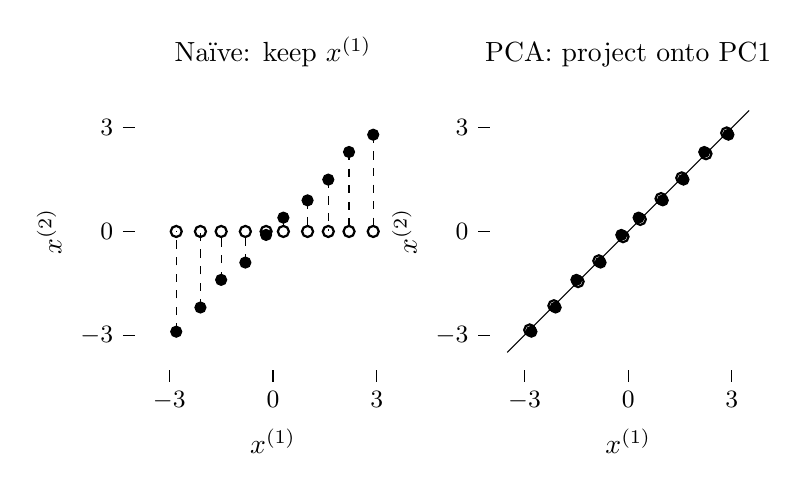
\begin{tikzpicture}
    \begin{axis}[
        name=naive,
        xlabel={$x^{(1)}$}, ylabel={$x^{(2)}$},
        xmin=-4, xmax=4,
        ymin=-4, ymax=4,
        width=0.42\textwidth,
        height=0.42\textwidth,
        axis line style={draw=none},
        tick style={black, thin},
        xtick={-3,0,3},
        ytick={-3,0,3},
        xticklabel style={font=\small},
        yticklabel style={font=\small},
        tick align=outside,
        tick pos=left,
        title={Na\"ive: keep $x^{(1)}$},
    ]
    % Data along y=x direction
    \addplot[only marks, mark=*, mark size=2pt, black] coordinates {
        (-2.8,-2.9) (-2.1,-2.2) (-1.5,-1.4) (-0.8,-0.9) (-0.2,-0.1)
        (0.3,0.4) (1.0,0.9) (1.6,1.5) (2.2,2.3) (2.9,2.8)
    };
    % Projection onto x-axis
    \addplot[only marks, mark=o, mark size=2pt, black, thick] coordinates {
        (-2.8,0) (-2.1,0) (-1.5,0) (-0.8,0) (-0.2,0)
        (0.3,0) (1.0,0) (1.6,0) (2.2,0) (2.9,0)
    };
    \foreach \xa/\ya in {-2.8/-2.9, -2.1/-2.2, -1.5/-1.4, -0.8/-0.9, -0.2/-0.1,
                          0.3/0.4, 1.0/0.9, 1.6/1.5, 2.2/2.3, 2.9/2.8}{
        \addplot[black, thin, dashed] coordinates {(\xa,\ya) (\xa,0)};
    }
    \end{axis}
    \begin{axis}[
        at={(naive.east)}, anchor=west, xshift=1cm,
        xlabel={$x^{(1)}$}, ylabel={$x^{(2)}$},
        xmin=-4, xmax=4,
        ymin=-4, ymax=4,
        width=0.42\textwidth,
        height=0.42\textwidth,
        axis line style={draw=none},
        tick style={black, thin},
        xtick={-3,0,3},
        ytick={-3,0,3},
        xticklabel style={font=\small},
        yticklabel style={font=\small},
        tick align=outside,
        tick pos=left,
        title={PCA: project onto PC1},
    ]
    % Same data
    \addplot[only marks, mark=*, mark size=2pt, black] coordinates {
        (-2.8,-2.9) (-2.1,-2.2) (-1.5,-1.4) (-0.8,-0.9) (-0.2,-0.1)
        (0.3,0.4) (1.0,0.9) (1.6,1.5) (2.2,2.3) (2.9,2.8)
    };
    % PC1 direction line
    \addplot[black, thin, domain=-3.5:3.5] {x};
    % Projections onto y=x line (project (a,b) onto y=x: ((a+b)/2, (a+b)/2))
    \addplot[only marks, mark=o, mark size=2pt, black, thick] coordinates {
        (-2.85,-2.85) (-2.15,-2.15) (-1.45,-1.45) (-0.85,-0.85) (-0.15,-0.15)
        (0.35,0.35) (0.95,0.95) (1.55,1.55) (2.25,2.25) (2.85,2.85)
    };
    \foreach \xa/\ya/\px/\py in {
        -2.8/-2.9/-2.85/-2.85, -2.1/-2.2/-2.15/-2.15, -1.5/-1.4/-1.45/-1.45,
        -0.8/-0.9/-0.85/-0.85, -0.2/-0.1/-0.15/-0.15,
        0.3/0.4/0.35/0.35, 1.0/0.9/0.95/0.95, 1.6/1.5/1.55/1.55,
        2.2/2.3/2.25/2.25, 2.9/2.8/2.85/2.85}{
        \addplot[black, thin, dashed] coordinates {(\xa,\ya) (\px,\py)};
    }
    \end{axis}
\end{tikzpicture}
\caption{Left: dropping $x^{(2)}$ projects onto the horizontal axis --- the dashed errors are large because the data varies along $y{=}x$, not along a coordinate axis. Right: PCA projects onto the direction of maximum variance; the reconstruction errors are tiny. Both features have nearly equal variance, so the na\"ive ranking cannot decide which to keep.}
\label{fig:naive_vs_pca}
\end{figure}

\newthought{Here both features have nearly the same variance,} so variance-based selection cannot decide which to keep.
Dropping either axis incurs large reconstruction error.
The real structure lies along the diagonal $y{=}x$, a direction that no original feature represents.

\newthought{The lesson:} selecting among existing axes is limited to cases where those axes already align with the data.
When the interesting variation runs between features, we need to construct new axes.
That is exactly what PCA does.


\section{Principal Component Analysis}\index{PCA}\index{covariance matrix}

\marginnote{\newthought{PCA}\cite{Pearson1901}\cite{Hotelling1933} finds orthogonal directions of maximum variance in the data.}

\newthought{Given centred data} $X \in \mathbb{R}^{n \times d}$, where rows are samples, PCA finds a $k$-dimensional subspace, $k < d$, that best represents the data.

\newthought{The variance maximization view.}
Find the direction $w_1 \in \mathbb{R}^d$ with $\|w_1\|{=}1$ that maximises the variance of projected data:

\begin{align*}
    w_1 &= \arg\max_{\|w\|=1} \text{Var}(Xw) \\
        &= \arg\max_{\|w\|=1} w^T \Sigma\, w
\end{align*}

where $\Sigma = X^T X / n$ is the covariance matrix.

\marginnote{\newthought{Lagrange multipliers.} Setting $\mathcal{L} = w^T \Sigma w - \lambda(w^T w - 1)$ and differentiating gives $\Sigma w = \lambda w$, so $w_1$ is the eigenvector of $\Sigma$ with the largest eigenvalue $\lambda_1$.}

\newthought{The solution:} $w_1$ is the eigenvector of $\Sigma$ corresponding to the largest eigenvalue $\lambda_1$.
The second principal component is the eigenvector with the second-largest eigenvalue, orthogonal to the first, and so on.
The first $k$ principal components together define the optimal $k$-dimensional subspace.

\newthought{The reconstruction error view.}
Equivalently, PCA minimises the squared reconstruction error:

\begin{align*}
    \min_{W \in \mathbb{R}^{d \times k},\; W^T W = I_k} \sum_{i=1}^n \|x_i - WW^T x_i\|^2
\end{align*}

Both views yield the same solution: the first $k$ eigenvectors of the covariance matrix.

\begin{figure}
\centering
\begin{tikzpicture}
    \begin{axis}[
        xlabel={$x^{(1)}$}, ylabel={$x^{(2)}$},
        xmin=-1, xmax=5,
        ymin=-1, ymax=4,
        width=0.5\textwidth,
        height=0.5\textwidth,
        axis line style={draw=none},
        tick style={black, thin},
        xtick={0,2,4},
        ytick={0,2},
        xticklabel style={font=\small},
        yticklabel style={font=\small},
        tick align=outside,
        tick pos=left,
    ]
    \addplot[only marks, mark=*, mark size=2pt, black] coordinates {(3,2.5)};
    \addplot[black, thin, domain=0:4] {0.8*x};
    \addplot[only marks, mark=o, mark size=2pt, black, thick] coordinates {(2.73,2.18)};
    \addplot[black, thin, dashed] coordinates {(3,2.5) (2.73,2.18)};
    \node[font=\small, anchor=west] at (axis cs:3.1,2.5) {$x$};
    \node[font=\small, anchor=north] at (axis cs:2.73,2.1) {$\hat{x}$};
    \node[font=\small, anchor=west] at (axis cs:2.9,2.3) {error};
    \end{axis}
\end{tikzpicture}
\caption{PCA projects $x$ onto the principal subspace (line), minimising the reconstruction error (dashed line to $\hat{x}$).}
\label{fig:pca_reconstruction}
\end{figure}


\begin{algorithm}[H]
\caption{PCA via Eigendecomposition}
\begin{algorithmic}[1]
\Require Centred data $X \in \mathbb{R}^{n \times d}$, target dimension $k$
\Ensure Principal components $W \in \mathbb{R}^{d \times k}$, projected data $Z \in \mathbb{R}^{n \times k}$
\State Compute covariance matrix $\Sigma = X^T X / n$
\State Compute eigendecomposition $\Sigma = V \Lambda V^T$
\State $W \gets$ first $k$ columns of $V$ (sorted by decreasing eigenvalue)
\State $Z \gets X W$ \Comment{Project data onto $k$-dimensional subspace}
\end{algorithmic}
\end{algorithm}

\newthought{Explained variance.}
The fraction of total variance explained by the first $k$ components is:

\begin{align*}
    \text{explained variance ratio} &= \frac{\sum_{i=1}^k \lambda_i}{\sum_{i=1}^d \lambda_i}
\end{align*}

Choose $k$ so that the cumulative explained variance exceeds a threshold, commonly 95\%.

\begin{marginfigure}
\centering
\begin{tikzpicture}
    \begin{axis}[
        xlabel={Components},
        ylabel={Cumulative variance},
        xmin=0, xmax=10,
        ymin=0, ymax=1.1,
        width=\marginparwidth,
        height=\marginparwidth,
        axis line style={draw=none},
        tick style={black, thin},
        xtick={0,5,10},
        ytick={0,0.5,0.95,1},
        xticklabel style={font=\tiny},
        yticklabel style={font=\tiny},
        tick align=outside,
        tick pos=left,
    ]
    \addplot[only marks, mark=*, mark size=2pt, black] coordinates {
        (1,0.6) (2,0.75) (3,0.85) (4,0.9) (5,0.93)
        (6,0.95) (7,0.97) (8,0.98) (9,0.99) (10,1.0)
    };
    \addplot[black, thin, dashed, domain=0:10] {0.95};
    \end{axis}
\end{tikzpicture}
\caption{Cumulative explained variance. The dashed line marks the 95\% threshold; six components suffice here.}
\label{fig:explained_variance}
\end{marginfigure}


\section{Singular Value Decomposition}\index{SVD}

\marginnote{\newthought{SVD} is the workhorse of numerical linear algebra and the computationally preferred route to PCA.}

Any matrix $X \in \mathbb{R}^{n \times d}$ has an SVD:

\begin{align*}
    X &= U \Sigma V^T
\end{align*}

where $U \in \mathbb{R}^{n \times r}$ holds orthonormal left singular vectors, $\Sigma \in \mathbb{R}^{r \times r}$ is diagonal with singular values $\sigma_1 \geq \sigma_2 \geq \ldots$, $V \in \mathbb{R}^{d \times r}$ holds orthonormal right singular vectors, and $r{=}\text{rank}(X)$.

\newthought{Connection to PCA.} The columns of $V$ are the eigenvectors of $X^T X$, with $\lambda_i = \sigma_i^2 / n$.
In practice, always compute PCA via the SVD: it is numerically stable and avoids forming $X^T X$ explicitly.

\newthought{Truncated SVD} keeps only the top $k$ singular values: $X_k = U_k \Sigma_k V_k^T$.
By the Eckart-Young-Mirsky theorem\cite{EckartYoung1936}, $X_k$ is the best rank-$k$ approximation to $X$ in both Frobenius and spectral norms.


\section{Independent Component Analysis}\index{ICA}

\marginnote{\newthought{ICA} seeks statistically independent sources, not just uncorrelated directions.}

\newthought{PCA finds uncorrelated components.}
ICA goes further and finds independent components\index{statistical independence}.

\newthought{The cocktail party problem.} Multiple microphones record a mixture of speakers.
Model: $X = AS$, where $A$ is a mixing matrix and $S$ contains independent source signals.
ICA estimates $W{=}A^{-1}$ to recover $S{=}WX$.

\newthought{The key insight:} independent non-Gaussian signals become more Gaussian when mixed, a consequence of the central limit theorem.
ICA maximises non-Gaussianity, measured via kurtosis or negentropy, to separate sources.
The FastICA\cite{Hyvarinen1999} algorithm implements this efficiently.


\section{t-SNE}\index{t-SNE}

\marginnote{\newthought{t-SNE} stands for t-distributed Stochastic Neighbour Embedding\cite{vanDerMaaten2008}. It is optimised for two- or three-dimensional visualization.}

\newthought{t-SNE preserves local structure}: nearby points in high dimensions stay nearby in the 2D embedding.
It does this in four steps.

\begin{algorithm}[H]
\caption{t-SNE}
\begin{algorithmic}[1]
\Require High-dimensional data $X$, perplexity, target dimension $k$
\State Compute pairwise similarities in high-D (Gaussian kernel): $p_{j|i} = \exp(-\|x_i - x_j\|^2 / 2\sigma_i^2) / \sum_{l \neq i} \exp(-\|x_i - x_l\|^2 / 2\sigma_i^2)$; symmetrize: $p_{ij} = (p_{j|i} + p_{i|j}) / 2n$
\State Initialize low-D embedding $Y$
\Repeat
    \State Compute low-D similarities with Student-$t$ kernel: $q_{ij} = (1 + \|y_i - y_j\|^2)^{-1} / \sum_{k \neq l} (1 + \|y_k - y_l\|^2)^{-1}$
    \State Gradient step: minimise $\text{KL}(P \| Q) = \sum_{ij} p_{ij} \log (p_{ij} / q_{ij})$
\Until{convergence}
\end{algorithmic}
\end{algorithm}

\newthought{Perplexity} controls the effective number of neighbours each point considers.
It sets the bandwidth $\sigma_i$ of the Gaussian kernel.
Typical values: 5--50.
Higher perplexity means more global structure is considered.

\marginnote{\newthought{Perplexity} is defined as $2^{H(P_i)}$ where $H$ is the Shannon entropy of the conditional distribution over neighbours. Think of it as the effective number of neighbours.}

\newthought{Interpreting t-SNE output} requires caution.

\begin{figure}
\centering
\begin{tikzpicture}
    \begin{axis}[
        name=low,
        title={Perplexity $= 5$},
        xmin=-30, xmax=30, ymin=-30, ymax=30,
        width=0.4\textwidth,
        height=0.4\textwidth,
        axis line style={draw=none},
        tick style={black, thin},
        xtick=\empty, ytick=\empty,
        tick align=outside,
        tick pos=left,
    ]
    \addplot[only marks, mark=*, mark size=1.5pt, black] coordinates {
        (-20,-15) (-18,-14) (-19,-16) (-21,-15)
        (0,0) (1,2) (-1,1) (2,-1)
        (15,20) (16,18) (14,19) (17,21)
    };
    \end{axis}
    \begin{axis}[
        at={(low.east)}, anchor=west, xshift=0.5cm,
        title={Perplexity $= 50$},
        xmin=-30, xmax=30, ymin=-30, ymax=30,
        width=0.4\textwidth,
        height=0.4\textwidth,
        axis line style={draw=none},
        tick style={black, thin},
        xtick=\empty, ytick=\empty,
        tick align=outside,
        tick pos=left,
    ]
    \addplot[only marks, mark=*, mark size=1.5pt, black] coordinates {
        (-15,-10) (-13,-8) (-14,-12) (-16,-9)
        (0,5) (2,7) (-2,6) (3,4)
        (12,15) (14,13) (11,14) (15,16)
    };
    \end{axis}
\end{tikzpicture}
\caption{Same data at two perplexity values. Cluster shapes, sizes, and between-cluster distances all change, neither reflects original geometry.}
\label{fig:tsne_perplexity}
\end{figure}

\newthought{Common pitfalls:}
\begin{itemize}
    \item Cluster sizes are meaningless: t-SNE equalises local densities.
    \item Distances between clusters are meaningless: the embedding preserves local, not global, structure.
    \item Results vary with random initialisation; run multiple times.
    \item t-SNE is for visualization only, not for preprocessing or downstream tasks.
\end{itemize}


\section{UMAP}\index{UMAP}

\marginnote{\newthought{UMAP} stands for Uniform Manifold Approximation and Projection\cite{McInnes2018}. It has theoretical foundations in Riemannian geometry and algebraic topology.}

\newthought{UMAP is a newer non-linear method} that typically preserves more global structure than t-SNE, runs faster on large datasets, and has a theoretical foundation in manifold learning.

\newthought{Key ideas.}
\begin{enumerate}
    \item Build a weighted $k$-nearest-neighbour graph in high dimensions.
    \item Find a low-dimensional embedding that preserves the graph structure.
    \item Use cross-entropy loss, rather than KL divergence, to match fuzzy simplicial sets.
\end{enumerate}

\newthought{Key parameters.} \texttt{n\_neighbors}, similar to perplexity and typically set between 15 and 200, controls how much local versus global structure is preserved.
\texttt{min\_dist}, typically 0.1--0.5, controls how tightly points cluster in the embedding.

\vspace{2.5em}

\newthought{Choosing a method} depends on what you want to preserve and what comes next.

\begin{table*}[ht]
\centering
\begin{tabular}{p{0.12\textwidth}p{0.1\textwidth}p{0.12\textwidth}p{0.45\textwidth}}
    \toprule
    \textbf{Method} & \textbf{Linear} & \textbf{Scalable} & \textbf{Best use} \\
    \midrule
    PCA   & Yes & Yes    & Preprocessing, denoising, linear structure \\
    ICA   & Yes & Yes    & Source separation, statistical independence \\
    t-SNE & No  & Medium & Visualization of small datasets ($n < 10\,000$) \\
    UMAP  & No  & Yes    & Visualization of large datasets, more global structure \\
    \bottomrule
\end{tabular}
\vspace{2em}
\caption{Comparison of dimensionality reduction methods. None of the non-linear methods are appropriate for preprocessing features for downstream learning.}
\label{tab:dim_reduction_methods}
\end{table*}


% ==============================================================================================
% BLOCK 3: STUDENT ACTIVATION
% ==============================================================================================

\newpage

\section{Examples \& Exercises}\index{examples}\index{exercises}

\newthought{Computing by hand} builds the geometric intuition that plotting the output never can.
Step through the arithmetic slowly.

\vspace{1em}

\newthought{Given centred data}
$X = \begin{pmatrix} 2 & 1 \\ 1 & 2 \\ -1 & -2 \\ -2 & -1 \end{pmatrix}$,
compute the covariance matrix $\Sigma$, find its eigenvalues and eigenvectors, and determine what fraction of variance PC1 explains.

The covariance matrix:
\begin{align*}
    \Sigma &= \frac{1}{4} X^T X \\
           &= \frac{1}{4} \begin{pmatrix} 10 & 8 \\ 8 & 10 \end{pmatrix} \\
           &= \begin{pmatrix} 2.5 & 2 \\ 2 & 2.5 \end{pmatrix}
\end{align*}

Eigenvalues from $\det(\Sigma - \lambda I) = 0$:
\begin{align*}
    (2.5 - \lambda)^2 - 4 &= 0 \\
    \lambda_1 &= 4.5 \\
    \lambda_2 &= 0.5
\end{align*}

Eigenvectors: $v_1 = (1,1)/\sqrt{2}$, $v_2 = (1,-1)/\sqrt{2}$.
Explained variance by PC1:
\begin{align*}
    \frac{\lambda_1}{\lambda_1 + \lambda_2} &= \frac{4.5}{5} \\
                                             &= 90\%
\end{align*}

Now derive the projection of each data point onto PC1 yourself, then verify that the projected points have variance $4.5$.

\vspace{2.5em}

\newthought{Choosing a threshold.} A dataset has eigenvalues: 100, 50, 20, 10, 5, 3, 2, 1, 0.5, 0.5 (total ${=}192$).
How many components explain 90\% of the variance?
How many for 99\%?
Sketch the cumulative explained variance curve and identify the elbow.

\marginnote{Cumulative sums: 100, 150, 170, 180, 185, 188, 190, 191, 191.5, 192.\\[4pt]90\% threshold: $\geq 172.8$, so 3 components.\\99\% threshold: $\geq 190.1$, so 7 components.}

\vspace{2.5em}

\newthought{t-SNE interpretation trap.} You run t-SNE on a dataset and observe: cluster A has diameter 10 units, cluster B has diameter 5 units, and the distance between clusters is 20 units.
What can you conclude?
What can you not conclude?

Think carefully: t-SNE preserves local neighbourhood, not global geometry.
Cluster sizes and between-cluster distances in the 2D plot tell you nothing about the original space.


% ============================= CODE ===============================

\marginnote{\newthought{Code} will be provided as a Python notebook.
Use it as a starting point, break things, and observe what changes.}

\newthought{A coffee aroma dataset to explore.}
You are given 200 aroma fingerprints in 50 dimensions, four brewing varieties.
Apply PCA, retaining enough components to explain 95\% of variance.
Scatter-plot the first two principal components, colour-coded by variety.
Run t-SNE and UMAP on the same data and compare the three embeddings.

\newthought{What to observe.}
PCA preserves global structure: the four varieties form elongated regions that reflect their actual distances in the original space.
t-SNE compresses each variety into a tight ball; distances between balls are arbitrary.
UMAP may show clearer cluster separation than t-SNE while better preserving global topology.
Reconstruction error from PCA tells you whether 50 dimensions were truly needed.


\section{Self-Reflection and Recap}\index{reflection}\index{recap}

\newthought{Self-Reflection} questions to guide your thinking:
\begin{itemize}
    \item What does it mean for data to have low intrinsic dimensionality?
    \item Why does PCA correspond to an eigenvector decomposition of the covariance matrix?
    \item What is the difference between an uncorrelated and an independent component?
    \item Why does t-SNE use a Student-$t$ kernel in the low-dimensional space but a Gaussian in the high-dimensional space?
    \item When would you prefer UMAP over t-SNE, and when would you use PCA instead of either?
    \item What does the perplexity parameter actually control, and what happens when it is too low or too high?
    \item Why should you never use t-SNE or UMAP embeddings as features for a downstream classifier?
    \item How does the curse of dimensionality motivate dimensionality reduction before running K-Means?
\end{itemize}

\newthought{Recap} of Key Concepts:
\begin{itemize}
    \item PCA finds the orthogonal directions of maximum variance via eigendecomposition of the covariance matrix; SVD is the numerically preferred implementation.
    \item The explained-variance ratio guides the choice of $k$; retain enough components to exceed a threshold such as 95\%.
    \item t-SNE and UMAP preserve local neighbourhood structure for visualization; cluster sizes and between-cluster distances in their output are not interpretable.
    \item ICA finds statistically independent sources by maximising non-Gaussianity, going beyond the uncorrelated directions found by PCA.
    \item No non-linear method should be used as a preprocessing step for downstream learning; use PCA or SVD for that purpose.
\end{itemize}

\marginnote{\newthought{The fundamental limit} of every method in this chapter: each input is mapped to a single point. There is no way to say how uncertain that mapping is, or to generate new plausible inputs by sampling from the compressed space.}

\newthought{PCA compresses each input to a single point.}
Given two coffee aroma profiles that differ only in a small measurement noise, their PCA projections land at two nearby points with no indication of how reliably they were placed there.
There is no principled way to generate a new profile by sampling from the compressed space, and no way to interpolate smoothly between two known profiles.

\marginnote{\newthought{Teaser.} Can we replace the single compressed point with a distribution, so that sampling from the latent space generates new, plausible data?}
\newthought{Variational Autoencoders} replace the single point with a distribution.
The encoder no longer outputs coordinates but outputs a mean and a variance, turning compression into probabilistic inference.
Every point in the latent space corresponds to something meaningful, and sampling from it generates new, plausible data.

\marginnote{\newthought{feedback}}
